\documentclass{article}

\usepackage[hidelinks]{hyperref}

\usepackage{tikz}
\usetikzlibrary{matrix,chains,positioning,decorations.pathreplacing,arrows}

\usepackage{minted}
\usemintedstyle{colorful}

\addtolength{\oddsidemargin}{-.875in}
\addtolength{\evensidemargin}{-.875in}
\addtolength{\textwidth}{1.75in}

\addtolength{\topmargin}{-.875in}
\addtolength{\textheight}{1.75in}

\bibliographystyle{plain}

\begin{document}

\title{An Exploration of Neural Networks as Applied to Written Language Classification}
\author{Erik Boesen, Candidate [Number]}
\maketitle

\begin{abstract}
We assess the extent to which artificial neural networks can be used to perform recognition of written languages (conveyed through standard Unicode text rather than as graphically recognized handwriting or type). We use an artificial deep neural network to achieve a success rate of [Insert] at distinguishing between 8 different languages following supervised training.
\end{abstract}

\section{Introduction}
In this research we seek to develop and implement (using C++) a neural network which differentiates between the world's 8 most common first languages according to \cite{ethnologue}, namely: Chinese, Spanish, English, Arabic, Hindi, Bengali, Portuguese, and Russian (ISO 639-1 alpha-2 codes zh, es, en, ar, hi, bn, pt, ru) \cite{iso639}.

\section{Technical stack}
For implementing our network we use C++. However, given that the general logic of the network could be implemented in practically any language, we use the most simplistic implementation possible; avoiding excessive use of C++-specific idioms. Any opaque logic is explained. Syntax highlighting is provided as well for ease of use:
\begin{minted}{cpp}
#include <iostream>

using namespace std;
int main(int argc, char *argv[]) {
    cout << "Hello world!" << endl;
}
\end{minted}

\subsection{Training Data}
To train our network, we use dumps of article contents in the selected languages from the Wikimedia Foundation, obtained from \cite{wikidumps} as recommended in \cite{langsamp}. % Remove second citation?

For each language, data was retrieved from the 2018-04-20 dump, using the format "Articles, templates, media/file descriptions, and primary meta-pages." These dump files are retrievable at \url{https://dumps.wikimedia.org/enwiki/20180420/enwiki-20180420-pages-articles.xml.bz2} (English, with the same URI format used for other languages). Chinese, Spanish, English, Portuguese, and Russian have Wikimedia databases too large to be practically handled; thus, we use only a single chunk of those databases, which are hosted at inconsistent URIs. We use a simple bash script to download and extract all data:
\inputminted{bash}{data/download.sh}

We then use a Python program \texttt{process.py} to extract article text from the raw XML files and parse it to remove markup characters \cite{parsewikixml}:
\inputminted{python}{data/process.py}

\section{A general overview of neural networks}
\subsection{Why use a Neural Network?}
Neural Networks are a common technique used in the burgeoning field of machine learning. Machine learning techniques are useful when a large and diverse set of data must be processed (often entailing categorization), but when writing explicit code to make distinctions between data points would be impractical. For example, when identifying objects in an image, as in \cite{hinton12}, it would be nearly impossible to write a procedure to directly read image data and distinguish between many images. Though there exist simpler machine learning techniques, such as the K Nearest Neighbors algorithm, these strategies have trouble making decisions in so many dimensions with such a complex output vector as demonstrated in \cite{knnic}. Though the concept of a neural network has existed since the 1980s [citation needed], they have recently had a resurgence of popularity. Machine learning techniques based on neural networks including deep learning [citation needed] and recurrent neural networks [citation needed] have recently been applied to diverse problems, including achieving victory over a human in the age-old game of Go [citation needed], differentiating between multiple thouands of different image classes \cite{hinton12}, and even recognizing voices [citation needed].

\subsection{Structure}
Neural Networks make tasks like the aforementioned easier by taking cues from neurobiology and simulating how a real brain makes decisions. In the brains of humans and other animals, many neurons are joined together. These neurons themselves simply take electrical input, adjust it, and pass it along to the next neuron. Biological brains readjust the behavior of their individual constituent neurons, and in doing so are able to perform the process of learning.

Though this is a gross oversimplification of the actual biological processes of learning and neuroplasticity, it may be a helpful metaphor to understand the function of an artificial neural network: the technique is remarkably similar, as you will see.

\subsubsection{A neuron}
The process performed by each neuron during training is relatively simple and is thus easier to think about independently. First, the neuron sums the output values of all previous neurons, including the bias neuron, multiplied by their weights. It then passes the result through an activation function, which brings the output into a regular range such as $(0, 1)$ or $(-1, 1)$. There exist many different activation functions, however, in this investigation we use the common $\sigma$ ("sigmoid") function:
$$\sigma(x)=\frac{1}{1+e^{-x}}$$

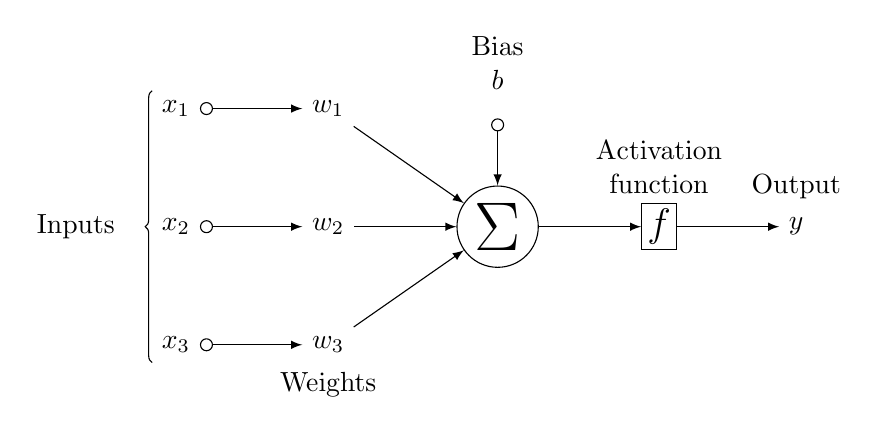
\begin{tikzpicture}[
init/.style={
  draw,
  circle,
  inner sep=2pt,
  font=\Huge,
  join = by -latex
},
squa/.style={
  draw,
  inner sep=2pt,
  font=\Large,
  join = by -latex
},
start chain=2,node distance=13mm
]
\node[on chain=2]
  (x2) {$x_2$};
\node[on chain=2,join=by o-latex]
  {$w_2$};
\node[on chain=2,init] (sigma)
  {$\displaystyle\Sigma$};
\node[on chain=2,squa,label=above:{\parbox{2cm}{\centering Activation \\ function}}]
  {$f$};
\node[on chain=2,label=above:Output,join=by -latex]
  {$y$};
\begin{scope}[start chain=1]
\node[on chain=1] at (0,1.5cm)
  (x1) {$x_1$};
\node[on chain=1,join=by o-latex]
  (w1) {$w_1$};
\end{scope}
\begin{scope}[start chain=3]
\node[on chain=3] at (0,-1.5cm)
  (x3) {$x_3$};
\node[on chain=3,label=below:Weights,join=by o-latex]
  (w3) {$w_3$};
\end{scope}
\node[label=above:\parbox{2cm}{\centering Bias \\ $b$}] at (sigma|-w1) (b) {};

\draw[-latex] (w1) -- (sigma);
\draw[-latex] (w3) -- (sigma);
\draw[o-latex] (b) -- (sigma);

\draw[decorate,decoration={brace,mirror}] (x1.north west) -- node[left=10pt] {Inputs} (x3.south west);
\end{tikzpicture}

Each neural network contains three types of layers, or vectors of neurons:
\begin{itemize}
\item{Input Layer - Neurons which directly recieve input values.}
\item{Hidden Layers - Input data is fed through one or more of these, which multiply values by various weights (notated $\omega_n$) in order to arrive at a final "output layer," which contains the data desired by a user.}
\item{Output Layer - A vector of output values.}
\end{itemize}

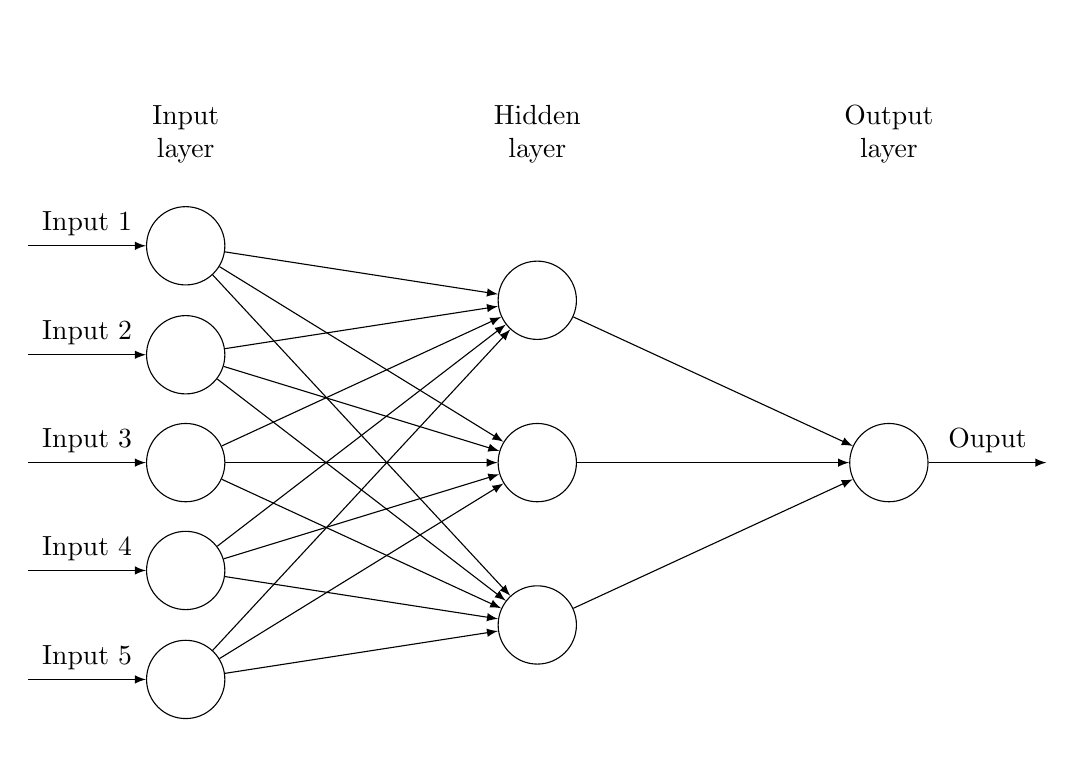
\begin{tikzpicture}[
plain/.style={
  draw=none,
  fill=none,
  },
net/.style={
  matrix of nodes,
  nodes={
    draw,
    circle,
    inner sep=10pt
    },
  nodes in empty cells,
  column sep=2cm,
  row sep=-9pt
  },
>=latex
]
\matrix[net] (mat)
{
|[plain]| \parbox{1.3cm}{\centering Input\\layer} & |[plain]| \parbox{1.3cm}{\centering Hidden\\layer} & |[plain]| \parbox{1.3cm}{\centering Output\\layer} \\
& |[plain]| \\
|[plain]| & \\
& |[plain]| \\
  |[plain]| & |[plain]| \\
& & \\
  |[plain]| & |[plain]| \\
& |[plain]| \\
  |[plain]| & \\
& |[plain]| \\    };
\foreach \ai [count=\mi ]in {2,4,...,10}
  \draw[<-] (mat-\ai-1) -- node[above] {Input \mi} +(-2cm,0);
\foreach \ai in {2,4,...,10}
{\foreach \aii in {3,6,9}
  \draw[->] (mat-\ai-1) -- (mat-\aii-2);
}
\foreach \ai in {3,6,9}
  \draw[->] (mat-\ai-2) -- (mat-6-3);
\draw[->] (mat-6-3) -- node[above] {Ouput} +(2cm,0);
\end{tikzpicture}

\subsection{Backpropogation}
A central component of neural network training is the backpropogation algorithm. In this

\bibliography{research}

\end{document}
